\documentclass[letterpaper, 12pt]{article}
\usepackage{fullpage}
\usepackage{cite}
\usepackage{graphicx}
\graphicspath{ {images/} }

\begin{document}

\title{Graph Isomorphism}
\author{Franklin van Nes}
\date{Tuesday 12th November, 2017}
\maketitle

\begin{enumerate}
    \item Formally define and describe the topic (whether technique, algorithm, model or class) in detail, and discuss its significance.
    \\
    Graph Isomorphism is most intuitively understood through its greek etymology: \textit{Iso}, meaning
     same, and \textit{morphism}, meaning shape; \textit{Graph Isomorhpism} $\rightarrow$ graphs that share the same shape.
    In more detail, two finite graphs are isomorphic if they share the same number of vertices connected in the same way.
    \\\\
    Formally, by an \textit{isomorphism} we mean from two graphs $G_1$ to $G_2$ we have a one-to-one mapping $f: G_1.V \rightarrow G_2.V$ from $G_1.V$ onto $G_2.V$ so
    that vertices $u_1$ and $v_1$ are adjacent in $G_1$ if and only if the vertices $f(u_1)$ and $f(v_1)$ are adjacent in $G_2$.
    If an isomorphism exists between $G_1$ and $G_2$, we say they are \textit{isomorphic}~\cite{gary-definer}.
    \\\\
     Graph isomorphism is also an equivalence relation which allows us to say that $G_1$ and $G_2$ are isomorhpic if they are equal, and they are equivalent if they are isomorphic.
    Figure \ref{graph-iso-image-figure} shows how two isomorphic graphs can look very different while still maintaining the same vertex adjacency.

    \item How do you show a problem is in the class?
    The class of problems within graph isomorphism is quite narrow. Determining graph isomorphism
    means given two graphs, determine if they are isomorphic. There also exists the \textit{Subgraph Isomorphism} problems
    where given $G_1$ and $G_2$,
    determine if $G_2$ is a subgraph of $G_1$. However, Subgraph Isomorphism, which is definitively NP-complete~\cite{cook1971complexity},
    is a generatlization of Graph Isomorphism, so we won't consider this in the same problem set as Graph Isomorphism.
    \\
    Many of the graph isomorphism algorithms
    can be used to determine subgraph isomorphism. However, it should be noted that determining
    Graph Isomorphism is complex in its own right. In fact, determining graph isomorphism falls
    into its own category of problem complexity, called \textit{Graph Isomorphism Complete}.
    According to Lubiw, it has yet to fall into a typical classification, and is neither P nor NP-complete~\cite{anna-complexity}.
    There exists no known P algorithm, yet graph isomorphism has not be shown to be NP-complete. This means that either a P algorithm
    must exist for graph isomorphism but it undiscovered, graph isomorhpism is a problem outside of
    P and NP, or, as Schöning argues, Graph isomorphism problems are in the low hierarchy of NP,
    which "does not equal NP unless the polynomial hierarchy collapses to the second level"~\cite{np-hierarchy}.
    Deeper explanation of this exceeds the reaches of this paper, though Schöning's research is well
    understood given the proper background knowlegdge.

    \item Which are representative or classic problems in this class?
    \\
    While there is really just one representative problem of this class - determine if two graphs are isomorphic -
    there are a large variety of consequential applications to solving this problem. For instance,
    database searches that use graphs instead of keywords. A great example of this is the biochecmical search
    engine described by Bonnici et al. . Given an unknown "biological networks at the molecular, protein, or species level",
    in a graph representation, how can we determine if it exists?
    edges of a graph. Attach any metadata, like bond angle, bond type and maybe the element of the atom.
    With that information, we can perform a graph isomoprhism against the database of graphs existing molecules
    to determine if our unknown molecule has previously been discovered and what it is commonly known as.
    Because this is such an expensive process, it would make sense to filter results on other criteria
    before determining graph isomorphism, or to use graph isomorphism algorithms to eliminate matches
    as quickly as possible to reduce the search space ~\cite{Bonnici2013}.
    \\
    Another application for graph isomorphism is with automata, to determine if two languages
    (perhaps represented by Turing Machine schema), are the same.

    https://math.stackexchange.com/questions/120408/what-are-the-applications-of-the-isomorphic-graphs
    \item How does this class compare to other classes?
    \item What techniques are used to solve problems in this class?

\end{enumerate}
\section{Figures}
\begin{figure}[h]
    \label{graph-iso-image-figure}
    \caption{Two isomorphic graphs. The colors indicate matching vertices, even
    if their labels do not match~\cite{wikimedia-images}}
    \centering
    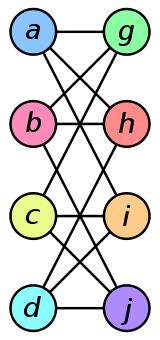
\includegraphics[scale=0.4]{graph-iso-a}
    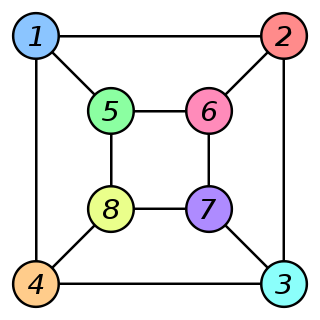
\includegraphics[scale=0.4]{graph-iso-b}
\end{figure}

\bibliography{mybib}{}
\bibliographystyle{abbrv}
\end{document}
